\documentclass{standalone}
\usepackage{tikz}
\usetikzlibrary{patterns, positioning}
\usepackage[sfdefault]{ClearSans} %% option 'sfdefault' activates Clear Sans as the default text font
\usepackage[T1]{fontenc}

\begin{document}
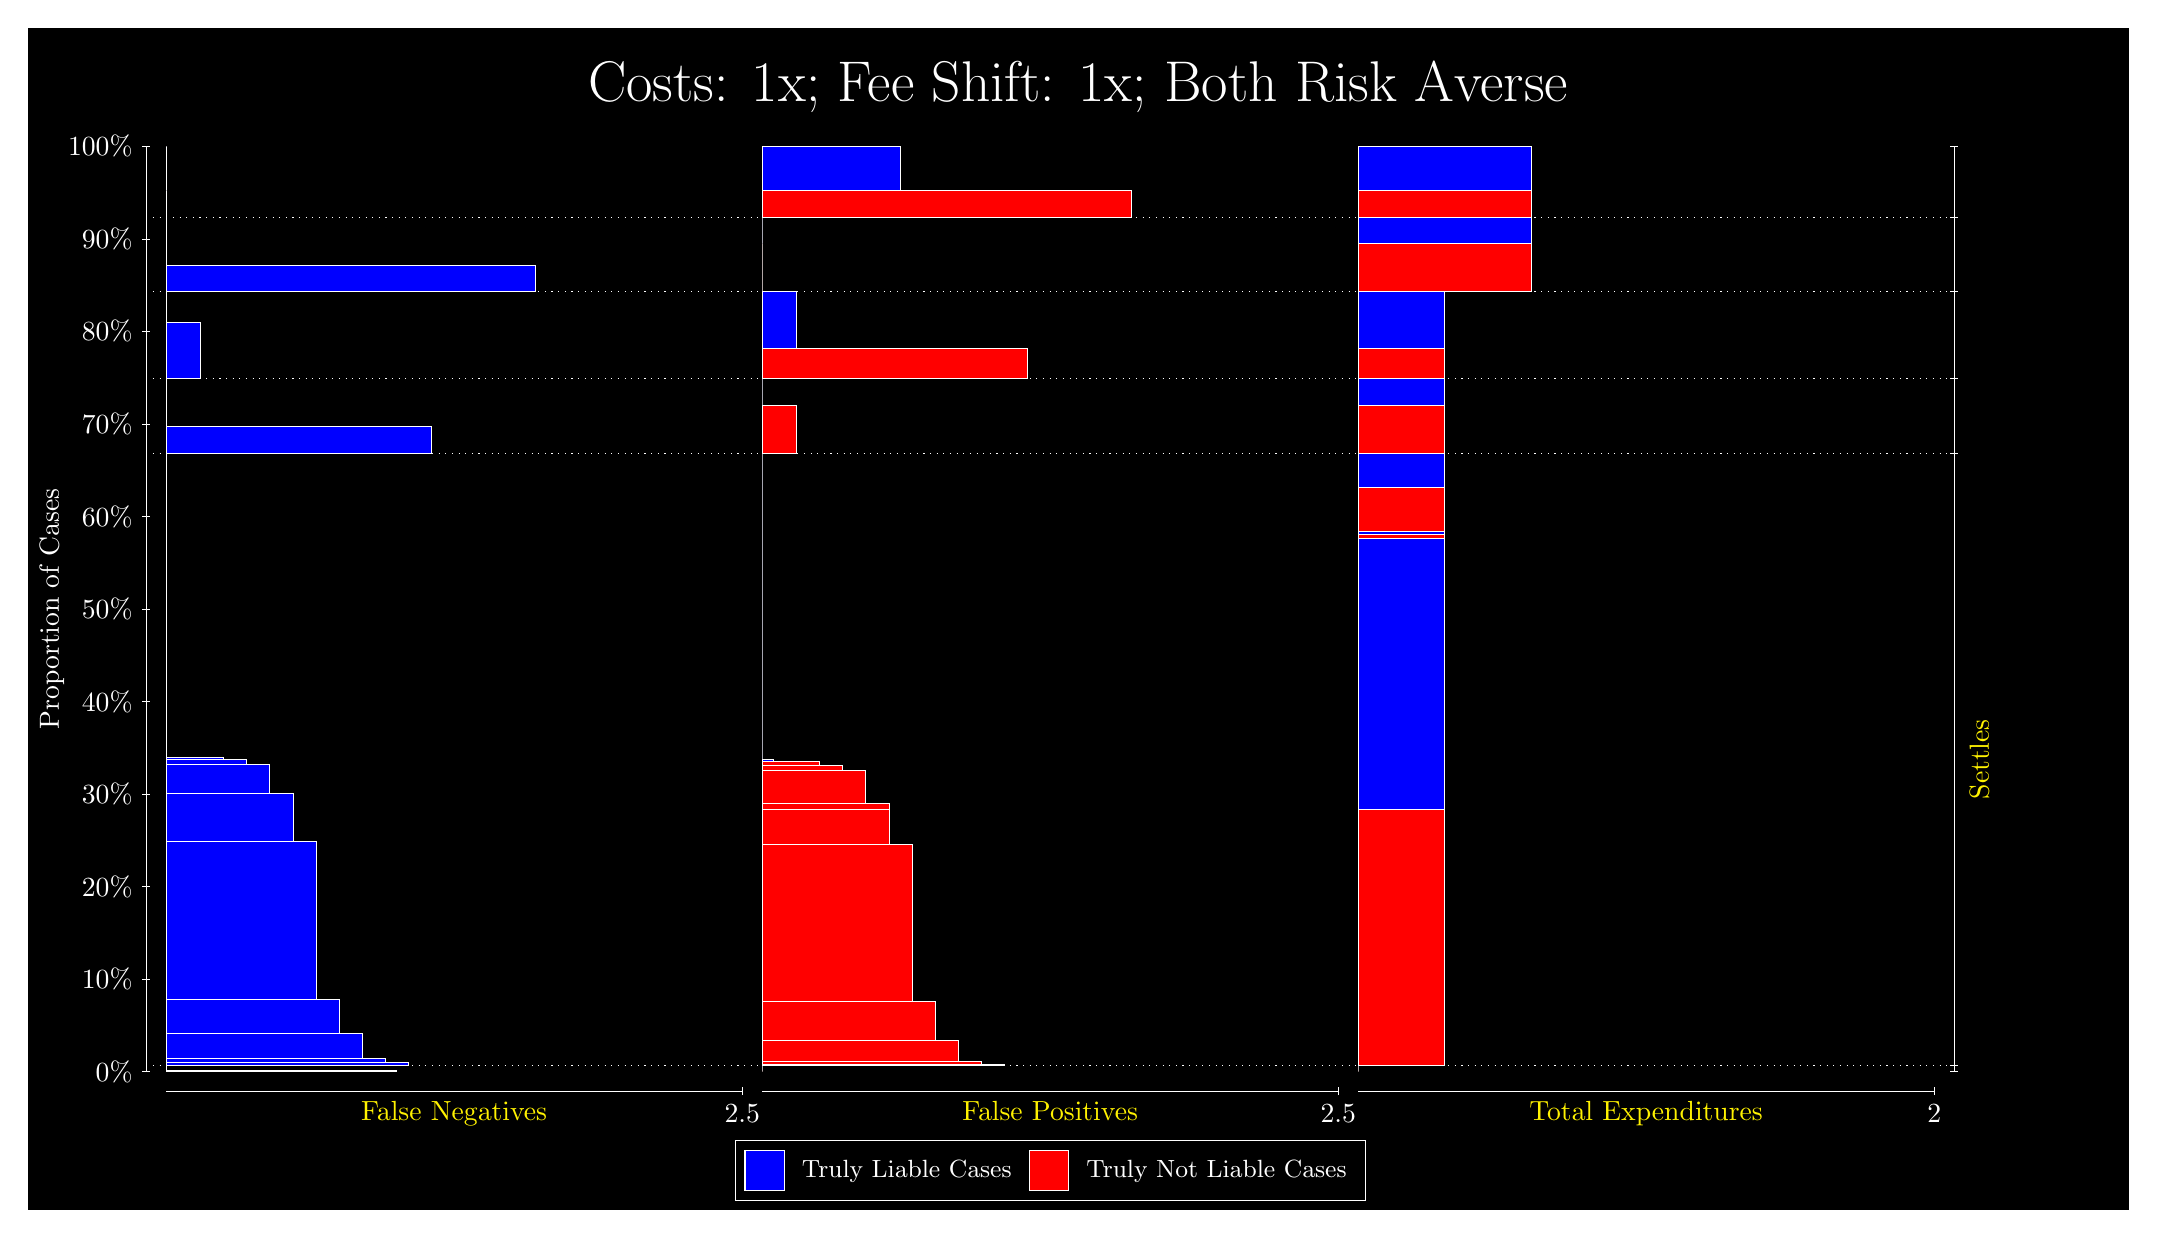
\begin{tikzpicture}
\draw[fill=black] (0,0) rectangle (26.667,15);
\draw[text=white] (0,13.5) rectangle (26.667,15) node[midway] {\huge Costs: 1x; Fee Shift: 1x; Both Risk Averse};
\draw[white, very thin] (1.5,1.75) -- (1.5,13.5);
\node[rotate=90, text=white, anchor=center] at (0.3, 7.625) {Proportion of Cases};
\draw[white, very thin] (1.45,1.75) -- (1.55,1.75);
\node[text=white, anchor=east] at (1.45, 1.75) {0\%};
\draw[white, very thin] (1.45,2.925) -- (1.55,2.925);
\node[text=white, anchor=east] at (1.45, 2.925) {10\%};
\draw[white, very thin] (1.45,4.1) -- (1.55,4.1);
\node[text=white, anchor=east] at (1.45, 4.1) {20\%};
\draw[white, very thin] (1.45,5.275) -- (1.55,5.275);
\node[text=white, anchor=east] at (1.45, 5.275) {30\%};
\draw[white, very thin] (1.45,6.45) -- (1.55,6.45);
\node[text=white, anchor=east] at (1.45, 6.45) {40\%};
\draw[white, very thin] (1.45,7.625) -- (1.55,7.625);
\node[text=white, anchor=east] at (1.45, 7.625) {50\%};
\draw[white, very thin] (1.45,8.8) -- (1.55,8.8);
\node[text=white, anchor=east] at (1.45, 8.8) {60\%};
\draw[white, very thin] (1.45,9.975) -- (1.55,9.975);
\node[text=white, anchor=east] at (1.45, 9.975) {70\%};
\draw[white, very thin] (1.45,11.15) -- (1.55,11.15);
\node[text=white, anchor=east] at (1.45, 11.15) {80\%};
\draw[white, very thin] (1.45,12.325) -- (1.55,12.325);
\node[text=white, anchor=east] at (1.45, 12.325) {90\%};
\draw[white, very thin] (1.45,13.5) -- (1.55,13.5);
\node[text=white, anchor=east] at (1.45, 13.5) {100\%};

\draw[white, very thin] (24.457,1.75) -- (24.457,13.5);
\draw[white, very thin] (24.407,1.75) -- (24.507,1.75);
\node[anchor=west] at (24.407, 1.75) {};
\draw[white, very thin] (24.407,1.8274) -- (24.507,1.8274);
\node[anchor=west] at (24.407, 1.8274) {};
\draw[white, very thin] (24.407,9.6029) -- (24.507,9.6029);
\node[anchor=west] at (24.407, 9.6029) {};
\draw[white, very thin] (24.407,10.55) -- (24.507,10.55);
\node[anchor=west] at (24.407, 10.55) {};
\draw[white, very thin] (24.407,11.655) -- (24.507,11.655);
\node[anchor=west] at (24.407, 11.655) {};
\draw[white, very thin] (24.407,12.595) -- (24.507,12.595);
\node[anchor=west] at (24.407, 12.595) {};
\draw[white, very thin] (24.407,13.5) -- (24.507,13.5);
\node[anchor=west] at (24.407, 13.5) {};

\draw[white, very thin, fill=blue] (1.75,1.75) rectangle (4.6775,1.7712);
\draw[white, very thin, fill=red] (1.75,1.7712) rectangle (1.75,1.8274);
\draw[white, very thin, fill=blue] (1.75,1.8274) rectangle (4.8239,1.8687);
\draw[white, very thin, fill=blue] (1.75,1.8687) rectangle (4.5312,1.9211);
\draw[white, very thin, fill=blue] (1.75,1.9211) rectangle (4.2384,2.2317);
\draw[white, very thin, fill=blue] (1.75,2.2317) rectangle (3.9457,2.6663);
\draw[white, very thin, fill=blue] (1.75,2.6663) rectangle (3.6529,4.6738);
\draw[white, very thin, fill=blue] (1.75,4.6738) rectangle (3.3602,5.2889);
\draw[white, very thin, fill=blue] (1.75,5.2889) rectangle (3.0674,5.6553);
\draw[white, very thin, fill=blue] (1.75,5.6553) rectangle (2.7746,5.7121);
\draw[white, very thin, fill=blue] (1.75,5.7121) rectangle (2.4819,5.7349);
\draw[white, very thin, fill=red] (1.75,5.7349) rectangle (1.75,9.6029);
\draw[white, very thin, fill=blue] (1.75,9.6029) rectangle (5.1167,9.9387);
\draw[white, very thin, fill=red] (1.75,9.9387) rectangle (1.75,10.55);
\draw[white, very thin, fill=blue] (1.75,10.55) rectangle (2.1891,11.271);
\draw[white, very thin, fill=red] (1.75,11.271) rectangle (1.75,11.655);
\draw[white, very thin, fill=blue] (1.75,11.655) rectangle (6.4341,11.983);
\draw[white, very thin, fill=red] (1.75,11.983) rectangle (1.75,12.595);
\draw[white, very thin, fill=red] (1.75,12.595) rectangle (1.75,12.939);
\draw[white, very thin, fill=blue] (1.75,12.939) rectangle (1.75,13.5);
\draw[white, very thin, fill=red] (9.3189,1.75) rectangle (9.3189,1.8061);
\draw[white, very thin, fill=blue] (9.3189,1.8061) rectangle (9.3189,1.8274);
\draw[white, very thin, fill=red] (9.3189,1.8274) rectangle (12.393,1.8447);
\draw[white, very thin, fill=red] (9.3189,1.8447) rectangle (12.1,1.8811);
\draw[white, very thin, fill=red] (9.3189,1.8811) rectangle (11.807,2.1442);
\draw[white, very thin, fill=red] (9.3189,2.1442) rectangle (11.515,2.6443);
\draw[white, very thin, fill=red] (9.3189,2.6443) rectangle (11.222,4.6298);
\draw[white, very thin, fill=red] (9.3189,4.6298) rectangle (10.929,5.0812);
\draw[white, very thin, fill=red] (9.3189,5.0812) rectangle (10.929,5.1628);
\draw[white, very thin, fill=red] (9.3189,5.1628) rectangle (10.636,5.5761);
\draw[white, very thin, fill=red] (9.3189,5.5761) rectangle (10.344,5.6393);
\draw[white, very thin, fill=red] (9.3189,5.6393) rectangle (10.051,5.6954);
\draw[white, very thin, fill=blue] (9.3189,5.6954) rectangle (9.4652,5.7181);
\draw[white, very thin, fill=blue] (9.3189,5.7181) rectangle (9.3189,9.6029);
\draw[white, very thin, fill=red] (9.3189,9.6029) rectangle (9.758,10.214);
\draw[white, very thin, fill=blue] (9.3189,10.214) rectangle (9.3189,10.55);
\draw[white, very thin, fill=red] (9.3189,10.55) rectangle (12.686,10.934);
\draw[white, very thin, fill=blue] (9.3189,10.934) rectangle (9.758,11.655);
\draw[white, very thin, fill=red] (9.3189,11.655) rectangle (9.3189,12.267);
\draw[white, very thin, fill=blue] (9.3189,12.267) rectangle (9.3189,12.595);
\draw[white, very thin, fill=red] (9.3189,12.595) rectangle (14.003,12.939);
\draw[white, very thin, fill=blue] (9.3189,12.939) rectangle (11.075,13.5);
\draw[white, very thin, fill=red] (16.888,1.75) rectangle (16.888,1.8061);
\draw[white, very thin, fill=blue] (16.888,1.8061) rectangle (16.888,1.8274);
\draw[white, very thin, fill=red] (16.888,1.8274) rectangle (17.986,5.0812);
\draw[white, very thin, fill=blue] (16.888,5.0812) rectangle (17.986,8.517);
\draw[white, very thin, fill=red] (16.888,8.517) rectangle (17.986,8.573);
\draw[white, very thin, fill=blue] (16.888,8.573) rectangle (17.986,8.6144);
\draw[white, very thin, fill=red] (16.888,8.6144) rectangle (17.986,9.1725);
\draw[white, very thin, fill=blue] (16.888,9.1725) rectangle (17.986,9.6029);
\draw[white, very thin, fill=red] (16.888,9.6029) rectangle (17.986,10.214);
\draw[white, very thin, fill=blue] (16.888,10.214) rectangle (17.986,10.55);
\draw[white, very thin, fill=red] (16.888,10.55) rectangle (17.986,10.934);
\draw[white, very thin, fill=blue] (16.888,10.934) rectangle (17.986,11.655);
\draw[white, very thin, fill=red] (16.888,11.655) rectangle (19.083,12.267);
\draw[white, very thin, fill=blue] (16.888,12.267) rectangle (19.083,12.595);
\draw[white, very thin, fill=red] (16.888,12.595) rectangle (19.083,12.939);
\draw[white, very thin, fill=blue] (16.888,12.939) rectangle (19.083,13.5);
\draw[white, dotted] (1.5,1.8274) -- (24.457,1.8274);
\draw[white, dotted] (1.5,9.6029) -- (24.457,9.6029);
\draw[white, dotted] (1.5,10.55) -- (24.457,10.55);
\draw[white, dotted] (1.5,11.655) -- (24.457,11.655);
\draw[white, dotted] (1.5,12.595) -- (24.457,12.595);
\draw[white, very thin] (1.75,1.5) -- (9.0689,1.5);
\node[text=yellow, anchor=north] at (5.4094, 1.5) {False Negatives};
\draw[white, very thin] (9.0689,1.45) -- (9.0689,1.55);
\node[text=white, anchor=north] at (9.0689, 1.45) {2.5};

\draw[white, very thin] (9.3189,1.5) -- (16.638,1.5);
\node[text=yellow, anchor=north] at (12.978, 1.5) {False Positives};
\draw[white, very thin] (16.638,1.45) -- (16.638,1.55);
\node[text=white, anchor=north] at (16.638, 1.45) {2.5};

\draw[white, very thin] (16.888,1.5) -- (24.207,1.5);
\node[text=yellow, anchor=north] at (20.547, 1.5) {Total Expenditures};
\draw[white, very thin] (24.207,1.45) -- (24.207,1.55);
\node[text=white, anchor=north] at (24.207, 1.45) {2};


\node[text=yellow, centered, rotate=90] at (24.777, 5.7151) {Settles};





\draw (12.978300999999998,1.5) node[draw=none] (baseCoordinate) {};
\begin{scope}[align=center]
        \matrix[scale=0.5, draw=white, below=0.5cm of baseCoordinate, nodes={draw}, column sep=0.1cm]{
            \node[rectangle, draw, minimum width=0.5cm, minimum height=0.5cm, fill=blue] {}; &
            \node[draw=none, font=\small, text=white] (B) {Truly Liable Cases}; &
            \node[rectangle, draw, minimum width=0.5cm, minimum height=0.5cm, fill=red] {}; &
            \node[draw=none, font=\small, text=white] (B) {Truly Not Liable Cases}; \\
            };
\end{scope}

\end{tikzpicture}
\end{document}